\documentclass[11pt, oneside]{article}   	% use "amsart" instead of "article" for AMSLaTeX format
\usepackage{geometry}                		% See geometry.pdf to learn the layout options. There are lots.
\geometry{letterpaper}                   		% ... or a4paper or a5paper or ... 
%\geometry{landscape}                		% Activate for for rotated page geometry
%\usepackage[parfill]{parskip}    		% Activate to begin paragraphs with an empty line rather than an indent
\usepackage{graphicx}				% Use pdf, png, jpg, or eps§ with pdflatex; use eps in DVI mode
								% TeX will automatically convert eps --> pdf in pdflatex		
\usepackage{amssymb}
\usepackage{amsmath}
\usepackage{parskip}
\usepackage{color}
\usepackage{hyperref}

\title{Complex function theory}
%\author{The Author}
%\section{}
%\subsection*{}
\date{}							% Activate to display a given date or no date

\graphicspath{{/Users/telliott_admin/Dropbox/Tex/png/}}
% \begin{center} 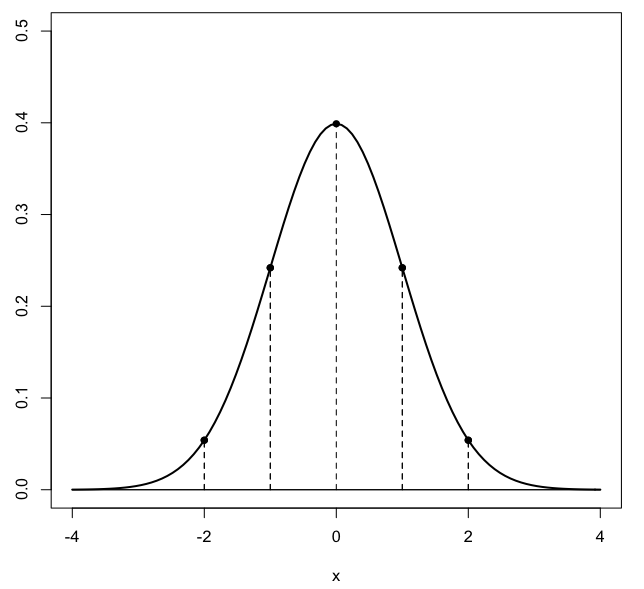
\includegraphics [scale=0.4] {gauss3.png} \end{center}
\begin{document}
\maketitle
\Large

Complex numbers arose in the context of finding solutions to certain polynomials, for example:
\[ x^2 + 1 = 0 \]
and
\[ x^2 + x + 1 = 0 \]
For the first equation, it is easy to see that there is no solution among the real numbers since $x^2$ is always positive or zero.  So adding $1 + x^2$ cannot bring the sum back to zero.

Visualizing the same function geometrically, this is just the simple parabola $y=x^2$ shifted up by one unit, moving its vertex from $(0,0)$ to $(0,1)$.  Plotting shows that the graphs of both functions never cross the $x$-axis---there are no values that lie on the curve and also on the line $y=0$.

The ingenious solution to this problem is to invent a new kind of number
\[ i = \sqrt{-1} \ , \ \ \ i^2 = -1 \]
Once we accept that $i = \sqrt{-1}$
then
\[ (x + i)(x - i) = x^2 - i^2 \]
\[ = x^2 - (-1) = x^2 + 1 \]
so $\pm \ i$ are both solutions to the equation 
\[ x^2 + 1 = (x + i)(x - i) = 0 \]
since if $x = i$ then $x - i = 0$ and if $x = -i$ then $x + i = 0$.

For the second one
\[ x^2 + x + 1 = 0 \]
we can plot it, or we can recall the quadratic formula for solutions to
\[ ax^2 + bx + c = 0 \]
for real constants $a$, $b$ and $c$.  The formula is
\[ \frac{-b \pm \sqrt{b^2 - 4ac}}{2a} \]
When $4ac > b^2$, then the solutions to the quadratic formula involve the square root of a negative number.  Here the formula gives
\[ \frac{-1 \pm \sqrt{-3}}{2} \]
Check the positive root:
\[ x^2 = (\frac{-1 + \sqrt{-3}}{2})^2 \]
\[ = \frac{1}{4} - \frac{\sqrt{-3}}{2} - \frac{3}{4} \]
Adding this to $x+1$ we obtain
\[  \frac{1}{4} - \frac{\sqrt{-3}}{2} - \frac{3}{4}  + \frac{-1 + \sqrt{-3}}{2} + 1 \]
the terms with $\sqrt{-3}$ cancel, giving
\[ = \frac{1}{4} - \frac{3}{4}  - \frac{1}{2} + 1 = 0 \]

In fact, now that we have $i$ available, any square root like $\sqrt{-(a^2)}$, where $a$ is a real number, can be factored as $\sqrt{-1} \ \sqrt{a^2} = ia$.

Note that the converse is not necessarily true.  Consider
\[ i^2 = \sqrt{-1} \cdot \sqrt{-1} \stackrel{?}{=} \sqrt{(-1)\cdot (-1)} = \sqrt{1} \]

Now, $\sqrt{1}$ has two solutions or roots (since $-1 \times -1$ and $1 \times 1$ are both equal to $1$), but we choose the positive root when thinking about $\sqrt{x}$ as a \emph{function}.  However, $i^2$ was defined to be equal to $-1$, not $1$.  What's the deal?

The problem is that the equality with a question mark is not valid
\[ \sqrt{-1} \cdot \sqrt{-1} \ne \sqrt{(-1)\cdot (-1)} \]
which explains why this "proof" is erroneous.

Expressions that involve the square root of a negative real number, like $\sqrt{-1} = i$ and $\sqrt{-3} = \sqrt{3}\ i$, are called imaginary (or \emph{purely} imaginary).  

Numbers that contain both a real and an imaginary part, like $1 + i$, are termed complex numbers, and imaginary numbers are considered to be complex numbers with the real part equal to $0$.

We say that the set of complex numbers $\mathbb{C}$ includes the real numbers:
\[ \mathbb{R} \subset \mathbb{C} \]

We write complex numbers $z$ as combinations like
\[ z = a + ib \]
 where $a$ and $b$ are both real numbers.  $a$ is the real part, and $b$ the imaginary part of the complex number $z$.

Some useful identities involving $i$ include
\[ i^2 = -1 \ , \ \ \  i = -\frac{1}{i} \ , \ \ \  -i = \frac{1}{i} \]

It turns out that for much of what is done with complex numbers the fact that $i$ equals $\sqrt{-1}$ is not even relevant.

Instead, we simply think of \emph{ordered pairs} of real numbers $(a,b)$ and the $i$ notation is a bookkeeping device, a marker to remind us that when we multiply two complex numbers
\[ (a + ib) (c + id) = ac + a \cdot id + ib \cdot c + ib \cdot id \]
the last term gets a minus sign:
\[ ib \cdot id = -bd \]
The result of multiplying $ib \cdot id$ is a real number with the sign flipped, while a real number $a$ times an imaginary number $id$ is equal to $iad$ and
\[ (a + ib) (c + id) = ac -bd + i(ad + bc) \]

Note carefully that if we consider two complex numbers $z_1 = a + ib$ and $z_2 = c + id$, then 
\[ z_1 = z_2 \iff a = c \text{ and } b = d \]
Two complex numbers $z_1$ and $z_2$ are equal \emph{if and only if} both the real and the imaginary parts are equal.

Another way to keep track of the same information is in matrix form, namely:
\[
z = \begin{bmatrix}
a & -b \\
b &  \ \ a
\end{bmatrix}
\]
Such matrices can be added and multiplied in the normal way and give the desired results for complex numbers.  Thus:
\[
\begin{bmatrix}
a & -b \\
b &  \ \ a
\end{bmatrix} \times
\begin{bmatrix}
c & -d \\
d &  \ \ c
\end{bmatrix} =
\begin{bmatrix}
ac + bd & -ad - bc \\
ad + bc &  \ \ ac + bd
\end{bmatrix} 
=
\begin{bmatrix}
 u & -v \\
v &  \ \ u
\end{bmatrix}
\]
\subsection*{Argand plane}
Yet another way to think about complex numbers is to use the complex plane (the Argand plane), where points are plotted with the real part along the horizontal axis and the imaginary part along the vertical axis.

This figure is from Brown \& Churchill.
\begin{center} 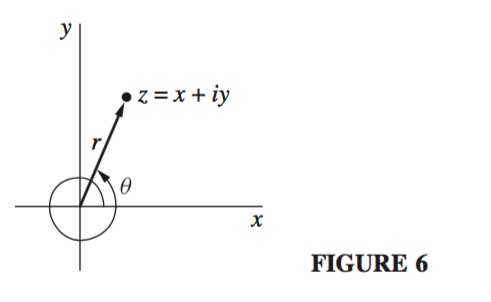
\includegraphics [scale=0.6] {Brown6.png} \end{center}

Looking at the graph, the distance of any point from the origin is denoted by $r$, and $\theta$ is the angle the ray makes with the positive $x$-axis in a CCW direction.  This should be familiar from standard polar coordinates.

Switching notation to
\[ z = x + iy \]
To plot the complex number $z$ we go out $x$ units along the real (horizontal) axis and then up $y$ units along the imaginary (vertical) axis.

The statement that $\mathbb{R} \subset \mathbb{C}$ is equivalent to the observation that the Argand plane contains the horizontal axis.  Real numbers have the form $z = x + i \cdot 0 = x$.

More generally, though
\[ x = r \cos \theta \]
\[ y = r \sin \theta \]
and
\[ x + iy = r \cos \theta + ir \sin \theta\]
\[ = r(\cos \theta + i \sin \theta) \]
\[ = re^{i\theta} \]
where the last part makes use of Euler's famous equation.  $r$ is called the \textbf{modulus} and $\theta$ is called the \textbf{argument} or \textbf{phase}.

Notice that in the figure above the argument $\theta$ is actually $\theta + 2 \pi$.  All multiples $k \cdot 2 \pi$ for $k \in 0, \pm 1, \pm 2 \dots$ are valid.

Calculations are often easier using one form rather than another.  Addition is simpler with $a + ib$ (the Cartesian format) since
\[ (a + ib) + (c + id) = (a+c) + i (b + d) \]
 while multiplication is more straightforward with the polar format.  Matrices work fine for both addition and multiplication.
 
Here is multiplication in polar coordinates
\[ r e^{i\theta} \ \rho e^{i\phi} = r \rho \ e^{i (\theta + \phi)} \]
We multiply the distances and add the angles.  Here is the square function:
\[ (r e^{i\theta})^2 = r^2 e^{i2\theta} \]

Multiplication of $z_1 = r_1 e^{i\theta_1}$ by $z_2 = r_2 e^{i\theta_2}$ stretches $r_1$ (the length of $z_1$) by the factor $r_2$ (the length of $z_2$), and rotates $z_1$ by adding a phase shift of $\theta_2$ to the original angle $\theta_1$.
\begin{center} 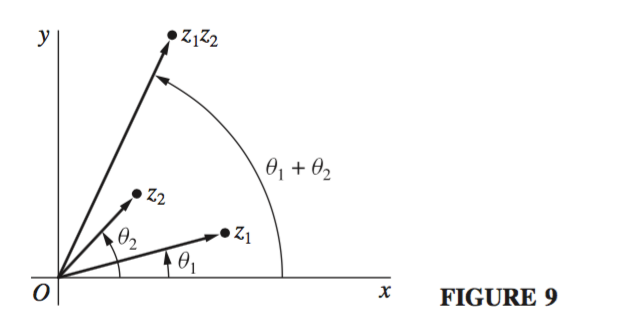
\includegraphics [scale=0.6] {Brown9.png} \end{center}

\end{document} 